\setmainfont{Noto Serif}
\setsansfont{Noto Sans}
\setmonofont{Noto Sans Mono}
\setstretch{1.35}

\section{Эффект Яна-Теллера}
1С. Используя теорию поля лигандов определите в каких из тетрахлорных комплексов $\text{[MeCl}_4]^{2-}$ кобальта, никеля и меди проявляется эффект Яна-Теллера. Для ян-теллеровских комплексов определите симметрию колебания, которое приводит к понижению симметрии.
\par
2С. В каких циклических системах возможен линейный эффект Яна-Теллера? Для случая циклопропиенильного радикала установите симметрию колебания, которое приводит к искажению геометрии. Определите также изменение полной электронной энергии данного радикала при понижении симметрии с $D_{3h}$ до $C_{2v}$. Считайте, что резонансные интегралы соответствующих связей изменились на 10\%.
\par
3. Определите проявляется ли эффект Яна-Теллера в молекулах $\text{BeH}_2$, $\text{CO}$.
\par
\begin{wrapfigure}{r}{25mm} %this figure will be at the right
    \centering
    \vspace{-2.6ex}
    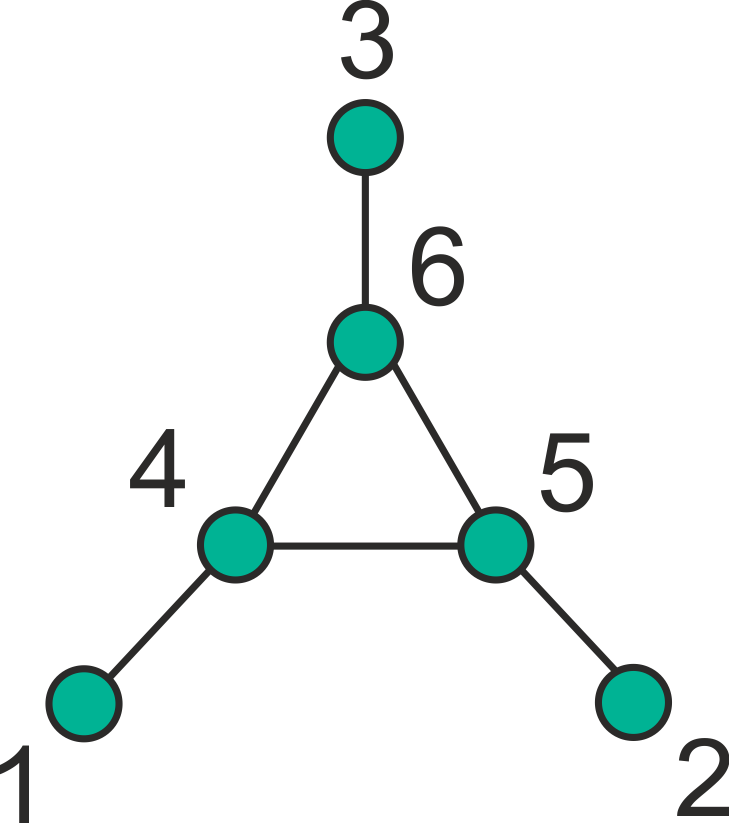
\includegraphics[width=16.5mm]{images/Fig_2_5_4.png}
    \vspace{-5ex}
\end{wrapfigure}
4С. Для какой формы (нейтральная молекула, катион-, анион-радикал) хюккелевской системы, изображенной на~рисунке может быть характерен эффект Яна-Теллера?
\par
5. Какова геометрия иона $\text{CH}_4^+$?
\par
6. Рассмотреть стабильность октаэдрических комплексов металлов с конфигурацией $d^1$–\,$d^{10}$ в высокоспиновом состоянии по отношению к эффекту Яна-Теллера.
\par
\begin{wrapfigure}{r}{45mm} %this figure will be at the right
    \centering
    \vspace{-4mm}
    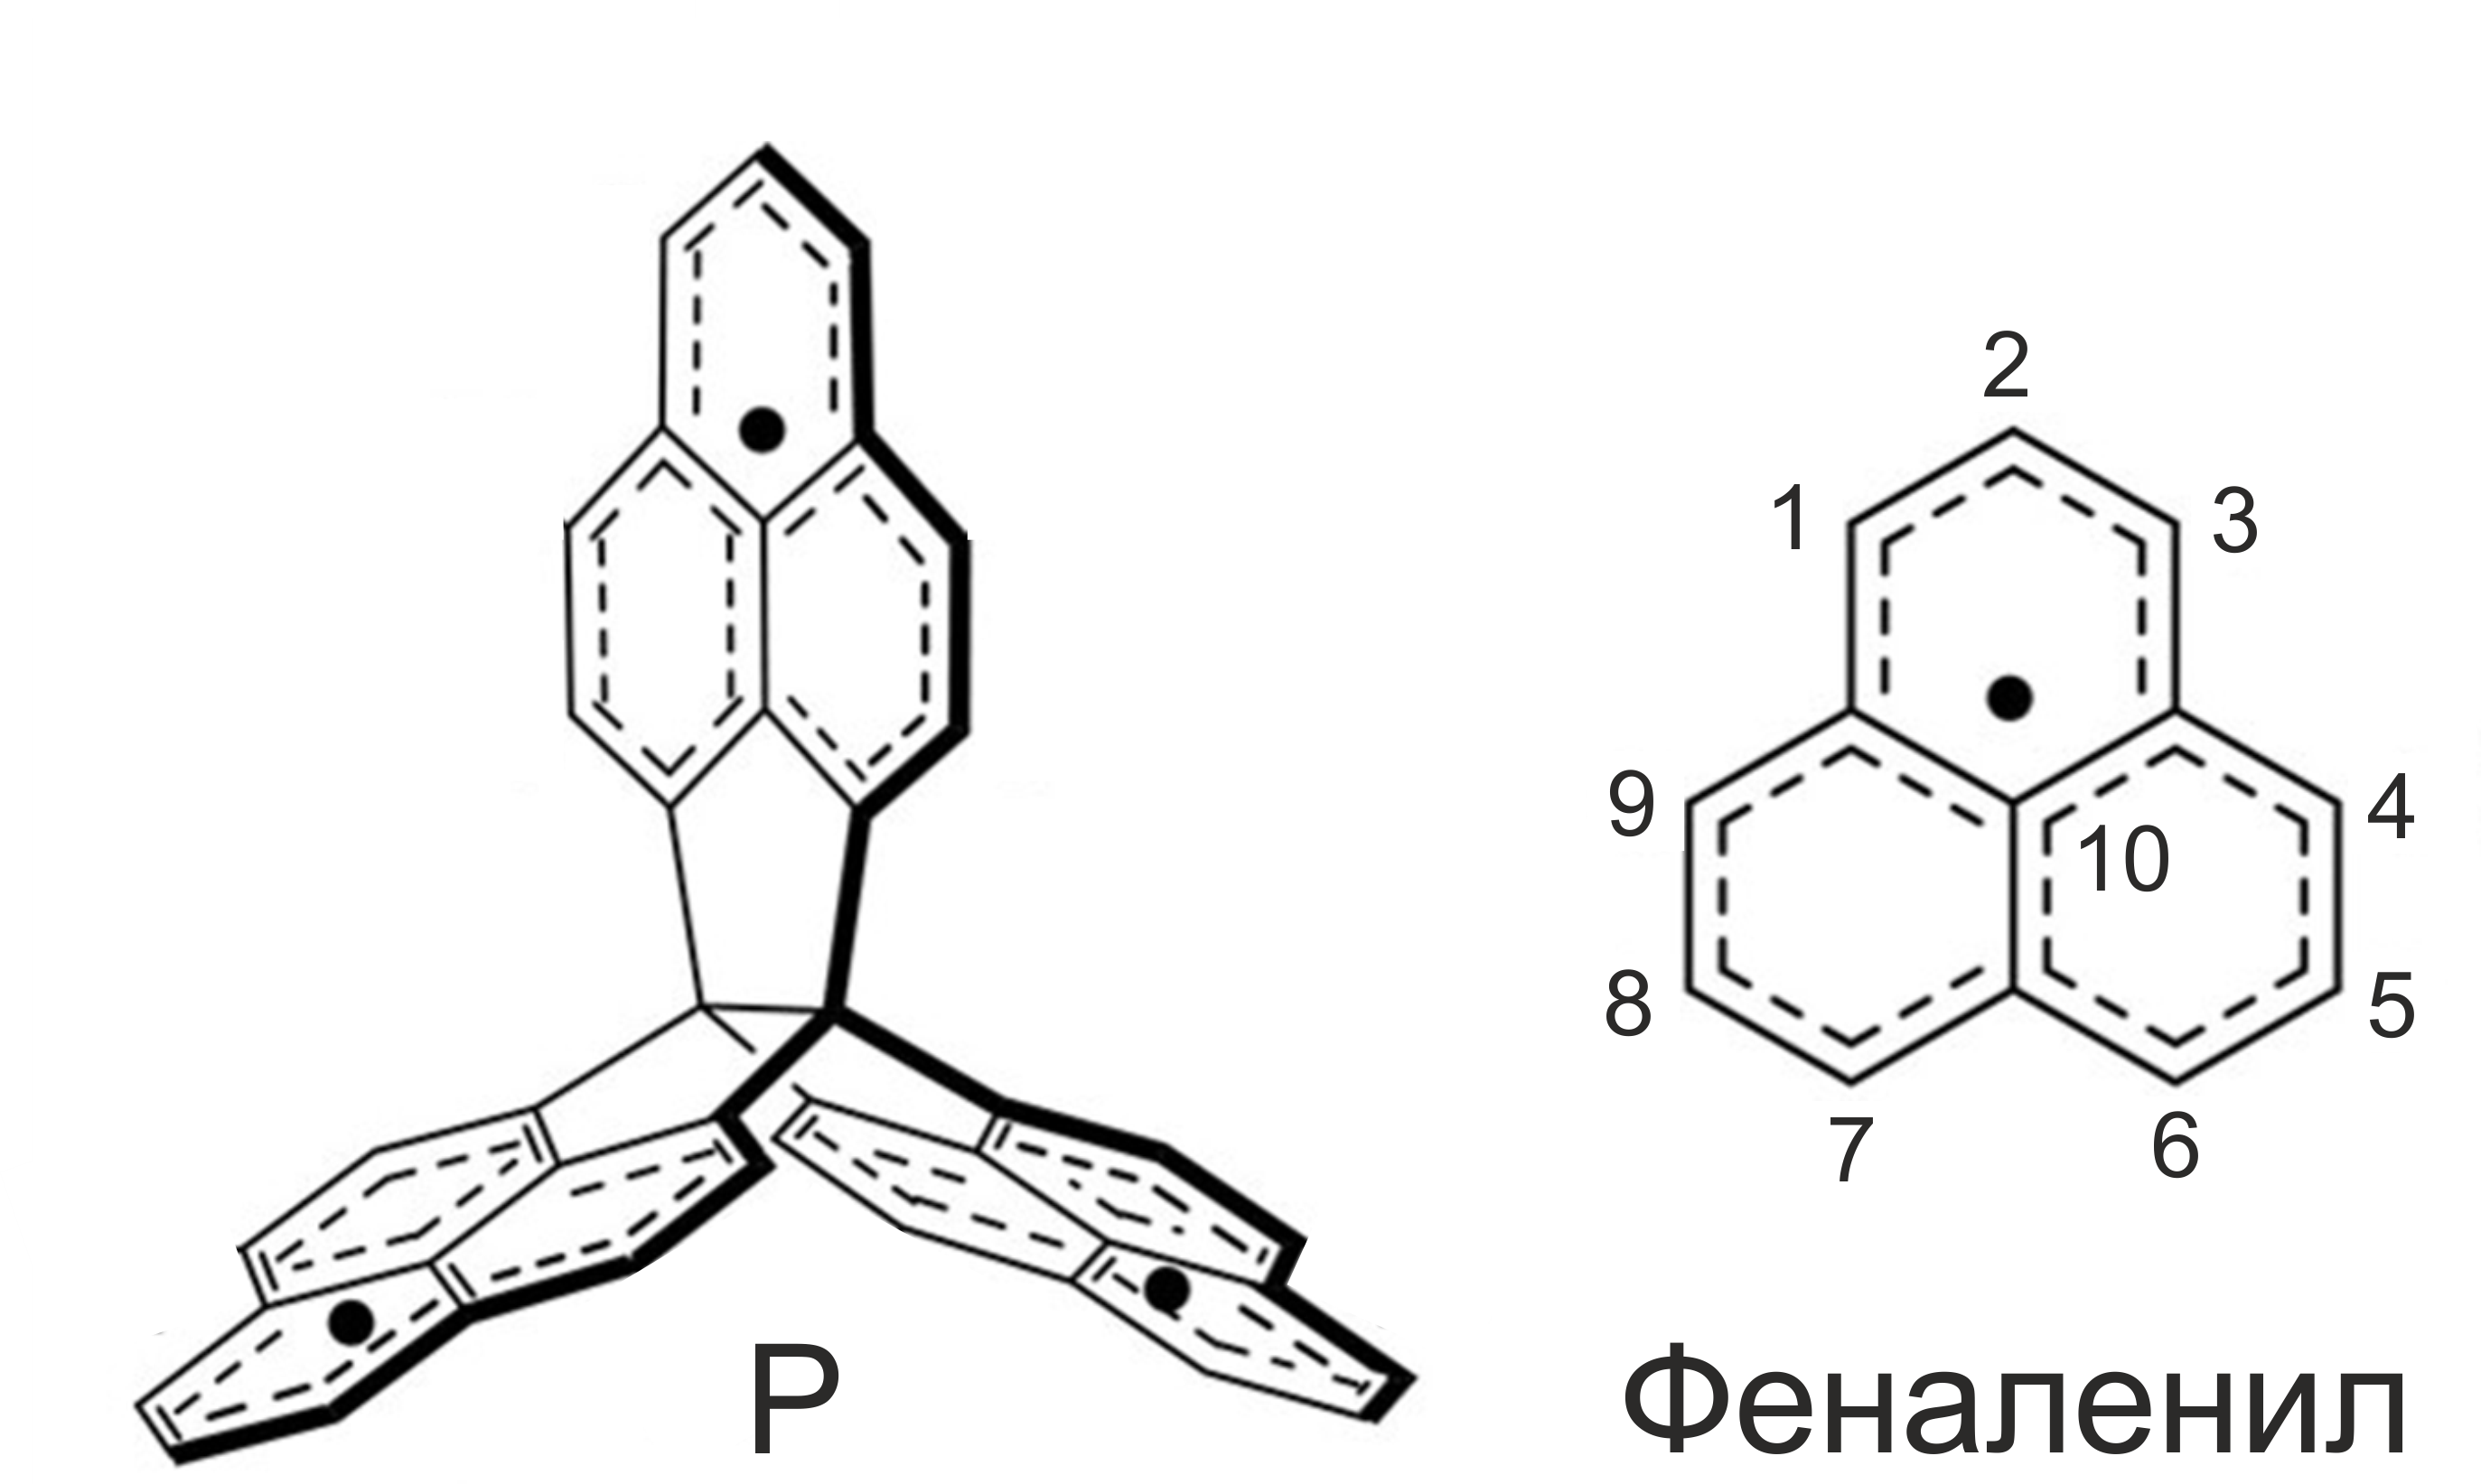
\includegraphics[width=45mm]{images/Fig_2_5_7.png}
    \vspace{-6mm}
\end{wrapfigure}
7К. В 2022 году японскими химиками был синтезирован пропеллероподобный трирадикал P на основе трех молекул феналенила. Структурные формулы P и феналенила приведены на рисунке справа. Используя однократно занятые молекулярные орбитали феналенила, определите вид и симметрию граничных молекулярных орбиталей трирадикала P, а также его основной терм. Подвержен ли P эффекту Яна-Теллера?
\par
8. Определите типы колебаний молекулы бензола, ответственные за такое перераспределение интенсивностей в его спектре поглощения, при котором за~счет разрешенного электронного перехода $A_{1g}$ $\rightarrow$ $E_{1u}$ возникают спектральные переходы $A_{1g}$ $\rightarrow$ $B_{1u}$ и $A_{1g}$ $\rightarrow$ $B_{2u}$.
\par
9. Показать, что для эффекта Яна-Теллера второго порядка существенны только колебания, симметрия которых совпадает с симметрией нижнего возбужденного состояния.
\par
